\chapter{Sensitivity to the Monopole Sky}

Now all that remains is actually answering the question of whether or not this 
could work.  Can a traditional interferometer actually pick up a global sky 
signal?  Can we manipulate that sensitivity using the strategic placement of 
absorptive materials around our antennas? And finally, and most importantly, 
can we actually understand the signals that we are sensitive to in order to 
accurately interpret our data, thereby actually observing the global signal of 
reionization?

\section{Simulated Visibilities}

Fundamentally, we are simply trying to calculate the visibility to the sky with 
a specific array set-up. We can describe this mathematically using the 
interferometric framework developed in Eq.~\eqref{eq:vis-allsky}. For the 
specific case we are investigating of a monopole sky and with absorptive 
baffles modifying the antenna beam, we get Eq.~\eqref{eq:vis-global-signal}:

\begin{equation}
 V(\nu) = T_{global}(\nu) \int A(\mathbf{s}) e^{-\tau(\mathbf{s,\nu})} e^{-2\pi 
 i \nu \mathbf{b}\cdot\mathbf{s}/c} ~d\mathbf{s}
    \label{eq:vis-global-signal}
\end{equation}

where $T_global$ is the temperature of the monopole sky, $A(\mathbf{S})$ is the 
antenna beam, $e^{-\tau(\mathbf{s})}$ is the spatial absorptivity, which is a 
function of direction and frequency. Here we see that the monopole sky has a 
convenient quality in that its lack of spatial information allows us to pull it 
out in front of the integral as a constant factor.

For our array, we will be considering the following set of perfectly east-west 
baseline separations: $\mathbf{b} = [0, \lambda/2, \lambda, 3\lambda/2, 
2\lambda, 3\lambda, 4\lambda]$ for a $\lambda = 100 MHz$.

Let's start by investigating the first question. Is an interferometer sensitive 
to the monopole sky? As described in Chapter~\ref{chap:logistics}, this can be 
be simulated, we just have to set our parameters appropriately.

We can begin with a very simplified proof-of-concept case. We will construct an 
array with no absorbers and a flat terrestrial horizon. Additionally, we will 
have beams with perfect receptivity in all directions, and a sky temperature of 
exactly $T_{global} = 1.0$ K across our entire observational band. This will be 
our most basic unit test -- something with which to check our intuition against 
and prove that the idea behind HYPERION is sound.

As expected and  as can be easily seen in 
Figures~\ref{fig:flat-sky-no-abs-freq} and~\ref{fig:flat-sky-no-abs-uv}, all 
ground-based interferometers have a non-zero sensitivity to the monopole mode 
of the sky. Similarly, we also find that the further we stray from the 
zero-spacing mode (i.e. as the number of wavelengths of separations increases), 
sensitivity to the monopole also quickly evaporates.

\begin{figure}
    \begin{center}
    \includegraphics[width=\linewidth]{/home/kara/documents/hyperion/memos/flat_sky_no_abs_freq.png}
    \end{center}
    \caption{
        Shown here is the absolute value of the visibility of a spectrally flat 
        monopole sky versus frequency. In this case, there are no absorptive 
        baffles, just the terrestrial horizon. As can be seen already, the 
        interferometer does have non-zero sensitivity to the monopole, though 
        it is plainly clear that the autocorrelation term (shown in blue) is 
        more sensitive than any of the non-zero interferometric baseline 
        pairings.
    }
    \label{fig:flat-sky-no-abs-freq}
\end{figure}

\begin{figure}
    \begin{center}
    \includegraphics[width=\linewidth]{/home/kara/documents/hyperion/memos/flat_sky_no_abs_uv.png}
    \end{center}
    \caption{
        Shown here is the absolute value of the visibility of a spectrally flat 
        monopole sky with no absorber walls versus uv-baseline. As can be seen 
        already, the interferometer has a non-zero sensitivity to the monopole 
        at non-zero baseline separations.
    }
    \label{fig:flat-sky-no-abs-uv}
\end{figure}

But this simple unit test tells us much more than just the fact that HYPERION 
is feasible after all. We can also begin to see a characteristic shape of the 
sensitivity in the \emph{uv}-plane, with peaks and nulls placed at regular 
intervals in \emph{uv}-space. The predictability of this shape could allow us 
to use it as a calibration tool, if properly understood. In particular, it 
could be a valuable way to remove leakage from non-monopole terms into our 
signal. Given that this characteristic shape derives only from the monopole sky 
and the shape of the beam, we know that any observational deviations in this 
shape must come from the sky rather than the system. Therefore, it may be 
possible to use this information as a way to filter out non-monopole terms from 
the sky, thus ensuring that we won't mix up spectral wiggles from the 
combination of various non-monopole sky sources with our expected wiggly 
reionization global signal, as seen in Fig.~\ref{fig:global-signal}. Instead, 
we can, effectively, select just the monopole terms of the sky -- the galactic 
synchrotron background and the reionization global signal -- thus ensuring that 
the only terms we're left with have simple relationships with frequency that 
can be easily parsed from the frequency-independent evolution of the 
reionization term.

Additionally, this characteristic shape could enable  us to do some weighting 
of our observational data. By knowing exactly what modes we expect to see the 
monopole term at its brightest and dimmest, we could properly weight and 
interpret data at each mode and frequency, enabling us to better compare data 
points at different points in \emph{uv}-space and frequency.

So we have established that we can detect the monopole with an interferometer, 
which is step one. But, as we can see, that sensitivity is faint, especially at 
the high-frequency end of our science band. That by itself is not wholly 
problematic -- we could just run our observation longer and beat down our 
sensitivity, assuming we still keep our spacing close enough that our 
observations don't have to run infinitely long. What is problematic is the 
strong cross-talk between elements that we know we'll face when we place them 
that close. We need to make our elements invisible to each other, and we think 
we can simultaneously enhance our sensitivity to the monopole as well.

In our next set of tests, we include the absorptive baffles around each 
antenna, as described in previous chapters. Using the absorption profile of the 
ferrite tiles, as seen in Fig.~\ref{fig:fe-absorption}, we can see how the 
monopole sensitivity is changed in the presence of the baffles.

As can be seen in Figures~\ref{fig:flat-sky-fe-abs-freq} 
and~\ref{fig:flat-sky-fe-abs-uv}, the sensitivity of the autocorrelation signal 
drops off, which is a nice sanity check on this test -- less signal from the 
sky getting picked up by the antenna means less bright visibility on the other 
end. However, while the spectral shape of the interferometric sensitivity 
changes, we don't see the same drop in sensitivity in the cross-correlation 
terms that we do in the auto-correlation. Moreover, as seen in 
Fig.~\ref{fig:flat-sky-fe-abs-freq}, we actually see \emph{increased} 
sensitivity at the high-frequency end of our science band.

\begin{figure}
    \begin{center}
    \includegraphics[width=\linewidth]{/home/kara/documents/hyperion/memos/flat_sky_with_fe_abs_freq_01.png}
    \end{center}
    \caption{
        Shown here is the absolute value of the visibility of a spectrally flat 
        monopole sky versus frequency, for an array with absorptive baffles 
        constructed from ferrite tiles. In comparison to 
        Fig.~\ref{fig:flat-sky-no-abs-freq}, we see that the reception of the 
        monopole signal has increased at higher frequencies. This indicates 
        that imposing the top-hat windowing function has indeed had the 
        intended effect of pushing the monopole sky into higher-order spatial 
        modes, increasing our array's sensitivity to the global signal.
    }
    \label{fig:flat-sky-fe-abs-freq}
\end{figure}

Additionally, we can see in Fig.~\ref{fig:flat-sky-fe-abs-uv} that the 
baselines no longer completely line up their peaks and nulls in $uv$-space.  
This is due to the frequency-dependent nature of the ferrite materials 
absorptive properties, as seen in Fig.~\ref{fig:fe-absorption}. If instead the 
ferrite had no variation in absorption across the science band, we would see a 
characteristic shape in $uv$-space that looked much more like 
Fig.~\ref{fig:flat-sky-no-abs-uv}, where all antenna pairs overlap cleanly in 
$uv$-space. This spatial-frequency variance makes it harder for us to 
calibrate, as we will have to compare the monopole measurements of each 
baseline only against matching baselines in the array, rather than by matching 
the measurements at each $uv$-coordinate in different baseline pairs. It would 
much better for our calibration and data processing purposes to be able to 
sample points of pure non-monopole foreground at multiple frequencies.  
Therefore, the project would benefit greatly from finding a way to even out the 
absorptivity of the baffles in frequency space.

\begin{figure}
    \begin{center}
    \includegraphics[width=\linewidth]{/home/kara/documents/hyperion/memos/flat_sky_with_fe_abs_uv_01.png}
    \end{center}
    \caption{
        Shown here is the absolute value of the visibility of a spectrally flat 
        monopole sky with ferrite absorber walls versus uv-baseline. We can see 
        that, in comparison to Fig.~\ref{fig:flat-sky-no-abs-uv}, the overall 
        shape of the characteristic monopole sensitivity is stretched in 
        $uv$-space, indicating that our imposed top-hat windowing function has 
        had the intended effect of pushing the monopole into higher order (and 
        more sensitive) spatial modes. However, we also see that the 
        sensitivity of the various baseline pairings of the array no longer 
        fall on top of one another. This is due to the frequency-dependent 
        nature of the ferrite as an absorber. Were we to find a way to even out 
        the absorptivity of the baffles in frequency, we would see that the 
        monopole sensitivities would also even out relative to each other, and 
        we would be better able to take advantage of the overlapping samples in 
        $uv$-space.
    }
    \label{fig:flat-sky-fe-abs-uv}
\end{figure}

\section{Recovered Global Signal}

Finally, we come to the question of whether or not we can accurately interpret 
our interferometric data in order to actually recover monopole sky, and in 
doing so observe the 21cm global signal of reionization. More to the point, we 
want to know if -- by knowing this characteristic monopole sensitivity at each 
frequency -- we can combine all of our data from the array, and each baseline 
separation pairing, and accurately recreate the true global signal.

To do this, we start by performing the exact same calculation described in 
Eq.~\eqref{eq:vis-global-signal} with a couple of key parameter changes. First 
off is that our $T_{global}$ is no longer a flat 1.0 K across all frequencies.  
instead, we import the ARES model of the 21cm reionization global signal, which 
is similar in its spectral behavior to 
Fig.~\ref{fig:global-signal}~\citep{mirocha2014}. We also construct our 
absorptive baffles out of ferrite tiles, i.e. using an absorption profile 
matching that of Fig.~\ref{fig:fe-absorption}. Additionally, we assume that 
there is a thermal, non-biased temperature to the system, with a flat value 
across our science band of $T_{sys} = 300$ K.  In order to beat down the noise, 
and in order to give ourselves a fighting chance of a detection, we also 
integrate for a total of 5 hours of observation over fifty 2 MHz channels, for 
a total of 100 MHz of observed bandwidth. All in all, this leaves an rms 
temperature in each frequency bin of about $T_{rms} = 
1.6$ mK, which should ensure that our 21cm reionization signal is plenty 
  visible. 

Finally, it is worth noting at this point that our array of antennas were 
arranged in a line, giving us a good set of redundant baselines. We took 
advantage of these duplicate measurements in this test, in order to give 
ourselves the best shot we could at (artificially) detecting the global signal.

We can combine all this data -- all the baselines and individual integrations 
over 5 hours and calculated monopole sensitivity coefficients -- by using a 
inverse-variance weighted average to invert our visibility into a brightness 
temperature.

Specifically, we will be using the characteristic monopole sensitivity 
coefficients as our weights in an inverse-variance weighting scheme. So, for 
example, looking at a non-redundant version of our array, for the same 
frequency bin we would have six different measurements of the visibility, 
$V(\nu) = [V_{\lambda/2}(\nu), V_{\lambda}(\nu), V_{3\lambda/2}(\nu), 
V_{2\lambda}(\nu), V_{3\lambda}(\nu), V_{4\lambda}(\nu)]$, where each 
visibility could be written as:

\begin{equation}
    V_i = w_i T_{global} + \sigma
    \label{eq:vis-weight}
\end{equation}

where $w_i$ is the value of the characteristic monopole sensitivity, 
$T_{global}$ is the aforementioned global sky temperature, and $\sigma$ is the 
expected value of the noise in each measurement. In order to recover an 
estimated value for the global sky temperature, we must find a way to write 
$T_{global}$ as a function of the measured visibility, the expected noise, and 
the weight of the measurement.  We can start by first isolating $T_{global}$ 
from its weight like so:

\begin{equation}
    \frac{V_i}{w_i} = T_{global} + \frac{\sigma}{w_i}
    \label{eq:isolated-temp}
\end{equation}

This seems promising, but we must recall that we do have some cases where the 
sensitivity of our measurement is very low (i.e. $w_i \ll 1$), resulting in a 
very large value of $\sigma/w_i$ in your estimate and causing problems. To 
solve this, we will implement an inverse-variance weighting scheme on our 
estimation, where the variance of the measurement would be:

\begin{equation}
    Var\Big(\frac{V_i}{w_i}\Big) = \frac{\sigma^2}{w_i^2}
    \label{eq:variance}
\end{equation}

Weighting our temperature measurement by this factor, we get a recovered 
temperature estimate of:

\begin{equation}
     \hat{T} = \frac{\sum \frac{V_i}{w_i} \frac{\sigma^2}{w_i^2}}{\sum 
     \frac{\sigma^2}{w_i^2}}
     \label{eq:measured-T}
\end{equation}

In the case that the expected noise of each measurement is the same (e.g. we 
would expect that the instrumental noise in the frequency bin would be the same 
in each measurement), then the noise term actually drops out and the above 
equation simplifies to become:

\begin{equation}
     \hat{T} = \frac{\sum V_i w_i}{\sum w_i^2}
     \label{eq:measured-T-simplified}
\end{equation}

And the variance on each measurement is given by:

\begin{equation}
    Var(\hat{T}) = \frac{\sigma^2}{\sum w_i^2} \sum \frac{1}{w_i}
    \label{eq:measured-T-variance}
\end{equation}

As can be seen in Fig.~\ref{fig:recovered-ferrite}, this method actually works!  
Our recovered temperature nearly perfectly recreates the true input signal, 
with small fluctuations in the brightness temperature only being introduced at 
high frequencies where the sensitivity is expected to be quite low as compared 
to the lower frequencies, as seen in Fig.~\ref{fig:flat-sky-fe-abs-freq}.

\begin{figure}
    \begin{center}
    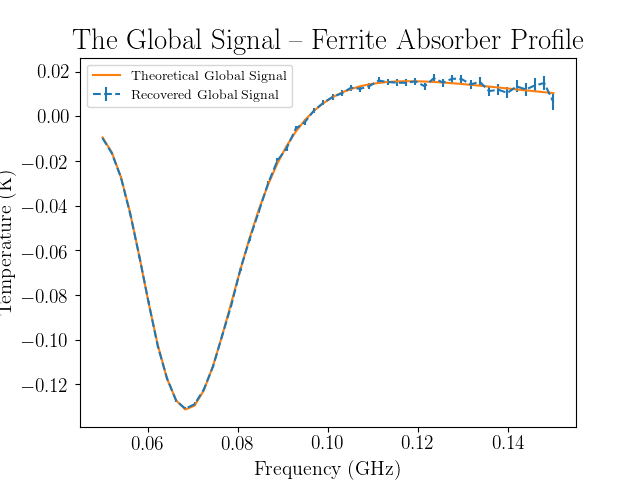
\includegraphics[width=\linewidth]{recovered_signal_same_abs.png}
    \end{center}
    \caption{
        Shown here is the recovered reionization global sky temperature, as 
        measured from a maximally redundant seven element east-west array with 
        a total integrated observation time of five hours, a flat system 
        temperature of $T_{sys} = 300$ K, and pure ferrite absorber baffles. As 
        can be seen, this method of observing the global sky temperature works 
        well, with nearly perfect recovery of the true monopole sky at low 
        frequencies (where our array has the highest sensitivities to the 
        monopole mode) and only small fluctuations (on the order of 3 mK) being 
        introduced at the low-sensitivity high-frequency end of our science 
        band. Although this is a highly idealized case, this is a positive 
        result, indicating that our method of weighting observations can 
        accurately recreate the true 21cm reionization global signal.
    }
    \label{fig:recovered-ferrite}
\end{figure}

Obviously this case is pretty idealized. Our thermal noise is unbiased and 
equal across all frequencies. Our sky is nothing but 21cm reionization monopole 
signal -- there is no galactic synchrotron emission nor spatial structure from 
other sources to account for. Our absorbers have been perfectly understood and 
characterized.

One thing we know about previous 21cm reionization global signal experiments is 
that their downfall comes from the fact that they are delicate. Every component 
of the experiment must be absolutely perfectly understood and calibrated in 
order to be successful, or their signal will be washed away with the 
systematics. So far, this has been an order too tall to be filled.

So what if we introduce a nit? What if something wasn't quite perfect with our 
array? What if, for instance, we didn't quite understand the nature of our 
absorber walls? In particular, what if we miscalibrated the absorptivity of the 
walls as a function of frequency?

In this case, we perform the exact same observation as above. However, where 
the data was actually collected using ferrite absorptive baffles, the 
calibration coefficients were calculated assuming a much simpler absorber 
model: one with a flat 15 dB absorptivity across the whole science band.  
Instead of having a monopole sensitivity like that seen in 
Fig.~\ref{fig:flat-sky-fe-abs-freq}, it looks like 
Fig.~\ref{fig:flat-sky-15dB-abs-freq}. So what happened to our recovered 21cm 
reionization temperature profile?

\begin{figure}
    \begin{center}
    \includegraphics[width=\linewidth]{/home/kara/documents/hyperion/memos/flat_sky_with_15dB_abs_freq_01.png}
    \end{center}
    \caption{
        Shown here is the absolute value of the visibility of a spectrally flat 
        monopole sky versus frequency, for an array with absorptive baffles 
        constructed from a material with a flat absorptivity of 15 dB across 
        the science band. Overall, this case that the lowest absolute 
        sensitivity to the monopole across the band, but it also has the 
        flattest slope for the drop-off in sensitivity, meaning the whole band 
        has relatively higher sensitivity if an observation is integrated just 
        a little while longer.
    }
    \label{fig:flat-sky-15dB-abs-freq}
\end{figure}

Good news! As can be seen in Fig.~\ref{fig:recovered-mismatched}, our recovered 
signal is still largely reflective of the true 21cm reionization global signal.  
The main difference seen comes at the low frequency end, where the recovered 
signal falls just slightly below the true signal up until a frequency of about 
80 MHz. In particular, we see that the main absorption feature of the signal is 
   slightly exaggerated, falling approximately 5 mK below the true signal.

\begin{figure}
    \begin{center}
    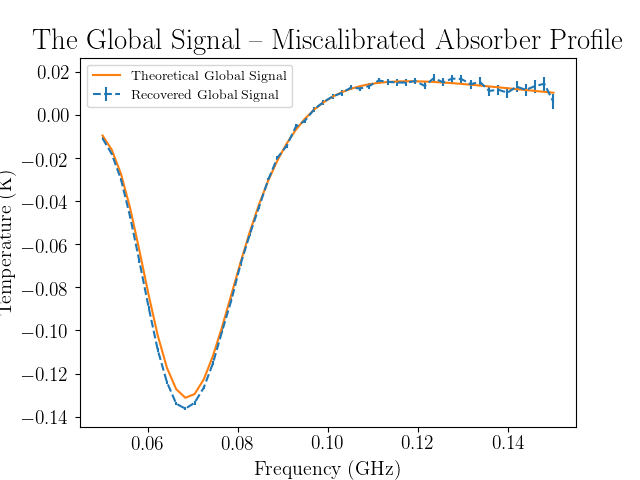
\includegraphics[width=\linewidth]{recovered_signal_diff_abs.png}
    \end{center}
    \caption{
        Shown here is the recovered reionization global sky temperature, as 
        measured from a maximally redundant seven element east-west array with 
        a total integrated observation time of five hours and a flat system 
        temperature of $T_{sys} = 300$ K. In this case, the data was collected 
        from an array using ferrite absorber baffles, but was calibrated 
        assuming the absorber baffles had a flat absorptivity of 15 dB across 
        the science band. As can be seen, even with this intentional gross 
        miscalibration of the system, we are still able to recreate a fairly 
        accurate portrayal of the true 21cm reionization global signal, with 
        the only major difference being a slight 5 mK exaggeration of the depth 
        of the absorption feature. This indicates that our weighting method is 
        robust to an imperfect calibration of the performance of the absorptive 
        baffles -- a promising result for the feasibility of the project.
    }
    \label{fig:recovered-mismatched}
\end{figure}

This is a promising initial result, indicating that the monopole interferometer 
may be more robust to minor calibration issues than its single-element 
counterparts may be. Our recovery isn't perfect in the case of a 
miscalibration, but it's still \emph{good} -- our features are still in the 
right places, the shapes are still there. No false spectral features have been 
introduced, suggesting reionization physics that contradicts the reality of the 
true 21cm reionization global signal.  This reassures us that even as we take 
our system into the backcountry and allow the elements to gently nudge all of 
our perfect lab calibration to the side, we have constructed a system strong 
enough to persist in giving us reasonably accurate answers. This result 
indicates that HYPERION may just have worked.
